\begin{intro}
  In order to study the mathematics not only of the Lamé-Navier
  equations but of more general systems of the form of
  equation~\eqref{eq:lame-navier-mixed}, we introduce abstract
  bilinear forms
  \begin{gather}
    \label{eq:mixedintro:1}
    \begin{aligned}
      a(u,v) &= 2\mu\form(\strain \vu, \strain \vu), &\vu,\vv&\in \vV \\
      b(u,p) &=  -\form(p,\div \vu), & \vu&\in \vV, p\in Q\\
      c(p,q) &= \tfrac1\lambda \form(p,q) & p,q&\in Q.
    \end{aligned}
  \end{gather}
\end{intro}

\begin{Definition}{saddle-point-operators}
  For each of the bilinear forms, we define associated operators
  \begin{gather}
    \begin{aligned}
      A&\colon V \to V^* & \scal(Au,v) &= a(u,v), \\
      B&\colon V \to Q^* & \scal(Bu,q) &= b(u,q), \\
      B^\transpose&\colon Q \to V^* & \scal(B^\transpose p,v) &= b(v,p), \\
      C&\colon Q\to Q^* & \scal(C p,q) &= c(p,q).
    \end{aligned}
  \end{gather}
  Here, $\scal(\cdot,\cdot)$ is the canonical pairing between an element of
  the dual space and the space itself.
\end{Definition}

\begin{Definition}{saddle-point-abstract}
  The abstract saddle-point problem in weak form reads: find a pair
  $(u,p)\in V\times Q$ such that
  \begin{gather}
    \label{eq:saddle-point-weak}
    \arraycolsep.1em
    \begin{matrix}
      a(u,v) &+& b(v,p) &=& f(v) &\quad&\forall v\in V, \\
      b(u,q) &-& c(p,q) &=& g(q) &&\forall q\in Q.
    \end{matrix}
  \end{gather}
  In operator notation, it reads
  \begin{gather}
    \label{eq:saddle-point-operator}
    \arraycolsep.1em
    \begin{matrix}
      Au &+& B^\transpose p &=& f &\quad&\text{in } V^*, \\
      Bu &-& C p &=& g &&\text{in } Q^*.
    \end{matrix}
  \end{gather}  
\end{Definition}

\begin{Notation}{saddle-point-form}
  We also consider the saddle-point system as a bilinear form $\mathcal A(\cdot,\cdot)$ on the space $X = V\times Q$, defined as
  \begin{gather}
    \mathcal A(x,y)
    = a(u,v) + b(v,p) + b(u,q) - c(p,q),
    \quad x =
    \begin{pmatrix}
      u\\p
    \end{pmatrix}
    ,\quad y=
    \begin{pmatrix}
      v\\q
    \end{pmatrix}
  \end{gather}
\end{Notation}

\begin{example}
  We clarify the denomination ``saddle-point system'' with a simple
  example: let $V = Q = \R$, and let $A=B=1$ as well as
  $C=0$. Choosing right hand side zero, we obtain the system
  \begin{gather}
    \mata \vx \equiv
    \begin{pmatrix}
      1 & 1 \\1 & 0
    \end{pmatrix}
    \begin{pmatrix}
      x_1 \\ x_2
    \end{pmatrix}
    =
    \begin{pmatrix}
     0\\0
    \end{pmatrix}
  \end{gather}
  Simple computation yields that $\vx\in \R^2$ solves this system if
  and only if $\vx$ is a stationary point of the \putindex{energy}
  $\nicefrac12\vx^\transpose\mata\vx$, namely
  \begin{gather}
    \nabla \left(\tfrac12\vx^\transpose\mata\vx\right) = 0.
  \end{gather}
  The shape of this energy as a function of $\vx$ is displayed in
  \cref{fig:saddle}. It resembles a saddle as known from horse riding
  or geography, hence the name.
\end{example}
\begin{figure}[tp]
  \centering
  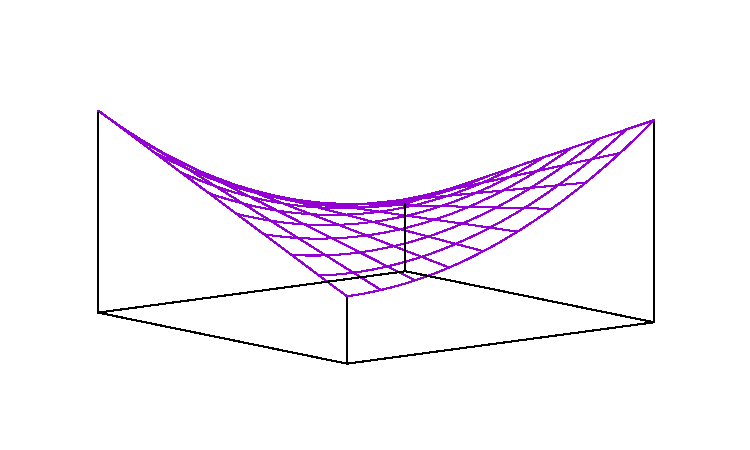
\includegraphics[width=.8\textwidth]{mixed/graph/saddle}
  \caption{The energy surface of a saddle-point system}
  \label{fig:saddle}
\end{figure}

\begin{Definition}{schur-complement}
  Let the operator $A:V\to V^*$ in the saddle-point system be
  invertible. Then, we define the \define{Schur complement} operator
  $S\colon Q\to Q^*$ of the system as
  \begin{gather}
      S= -B A^{-1} B^\transpose - C.
  \end{gather}
\end{Definition}

\begin{Lemma}{schur-complement1}
  Formally, the saddle-point system~\eqref{eq:saddle-point-operator}
  can be solved in two steps by solving
  \begin{align}
    S p &= g - B A^{-1} f,\\
    A u &= f-B^\transpose p.
  \end{align}
\end{Lemma}

\begin{proof}
  Formally solve the first equation
  of~\eqref{eq:saddle-point-operator} for $u$ and enter into the
  second.
\end{proof}

\begin{Lemma}{schur-definiteness}
  Let $a(\cdot,\cdot)$ be symmetric, positive definite such that
  $\tilde a(\cdot,\cdot) = \scal(A^{-1}\cdot,\cdot)$ is positive
  definite. Let $c(\cdot,\cdot)$ be positive semi-definite.  If
  $\ker{B^\transpose} + \ker C \neq Q$, then, the bilinear form
  $\mathcal A(\cdot,\cdot)$ is indefinite.
\end{Lemma}

\begin{proof}
  First, we note that because of ellipticity of $a(\cdot,\cdot)$
  \begin{gather}
    \mathcal A\mixedform(u,0,u,0) = a(u,u) \ge \gamma \norm{u}_V^2,
  \end{gather}
  for some positive constant $\gamma$. Furthermore, $A$ is invertible
  and its inverse is positive definite. Furthermore,
  $A^{-1}B^\transpose\colon Q\to V$. Then, choosing $v=-A^{-1}B^\transpose p$ yields
  \begin{align}
    \mathcal A\mixedform(v,p,v,p)
    &= a(A^{-1}B^\transpose p,A^{-1}B^\transpose p) - 2b(A^{-1}B^\transpose p,p) - c(p,p) \\
    &= \scal(B^\transpose p,A^{-1}B^\transpose p) - 2\scal(B^\transpose p,A^{-1}B^\transpose p) - c(p,p)\\
    &= -\scal(B^\transpose p,A^{-1}B^\transpose p) - c(p,p).
  \end{align}
  The first term is a quadratic term with the bilinear form associated
  with $A^{-1}$, which is positive definite. Thus, it is zero
  if and only if $B^\transpose p=0$, otherwise it is negative. The
  second term is negative unless $Cp=0$. By the assumption on the
  kernels of $B^\transpose$ and $C$ there exists $p$ such that at
  least one of the terms is nonzero. Therefore, we have found a
  vector such that
  \begin{gather}
    \mathcal A\mixedform(v,p,v,p) < 0.
  \end{gather}
\end{proof}

\begin{remark}
  The previous result holds in particular for
  $c(\cdot,\cdot) \equiv 0$, if $B^\transpose$ is injective.
\end{remark}

\begin{Problem}{saddle-unique-solution}
  Let $\mata \in \R^{n\times n}$ be a symmetric, positive definite
  matrix, $C\in \R^{m\times m}$ symmetric, positive
  semi-definite. Furthermore, let $B \in \R^{m\times n}$. Define the matrix
  \begin{gather}
    \mathscr A= 
    \begin{pmatrix}
      \mata & \matb^\transpose \\ \matb & -\matc
    \end{pmatrix}
    \in \R^{(m+n)\times (m+n)}
  \end{gather}
  \begin{enumerate}
  \item Show that the system $\mathscr A \vx = \vy$ has a unique
    solution for each $\vy$ (and thus $\mathscr A$ is invertible) if
    and only if
    \begin{gather}
      \ker{\matb^\transpose} \cap \ker \matc = \{0\}.
    \end{gather}
    Hint: consider the eigenvalues of the Schur complement.
  \item Let $\matc = 0$. Show that $\mathscr A$ is invertible if and
    only if $\matb$ is onto (surjective). Hint: theorem from linear
    algebra.
  \item Show that both hold if you relax the definiteness of $\mata$ to
    positive definite on $\ker \matb$.
  \end{enumerate}
\end{Problem}

%%% Local Variables: 
%%% mode: latex
%%% TeX-master: "main"
%%% End: 
